\documentclass{article}
\usepackage{geometry}
\geometry{legalpaper, margin=1in}
\usepackage[utf8]{inputenc}
\usepackage{hyperref}
\usepackage{graphicx}
\hypersetup{
    colorlinks=true,
    linkcolor=blue,
    filecolor=magenta,
    urlcolor=cyan,
}


\title{User Manual for the InifiniTag Document Tagging Service}
\author{Barnhill, Hanif, Vinokour, Wich, Sakib}
\date{June 2020}

\begin{document}

\maketitle
\tableofcontents

\newpage

\section{Introduction}
This documentation is aimed at the user attempting to use the InfiniTag software. The prerequesites
for this documentation are:

\begin{enumerate}
    \item The Solr database has already been setup
    \item The back end has been installed with the requirements
    \item The front end has been setup and is running.
\end{enumerate}

\bigskip
\noindent
For instructions on getting the front and back ends set up, see the \href{https://github.com/AMOS-5/infinitag/blob/master/README.md}{README} in the repository.

\bigskip
\noindent
For help getting the Solr database up and running. See the various files in our \href{https://github.com/AMOS-5/infinitag/tree/master/docs/solr}{Solr documentation}.



\section{Document Overview / Start Page}
\label{docoverview}
Once the front end is up and running, navigate to the start page to see a table with a list of documents as seen in Figure \ref{fig:start_page}.

Notice in the top right corner is a status badge indicating the connection to the back end. If this is 'DOWN', then you will not be able to send or receive information from the server and will not be able to continue.

The search bar on this page enables you to filter documents by any criteria. Any word entered into the search box will be used to check for matching words in the name, tags, language, etc.

The + icon in the keywords column allows you to add any existing tag to a document.

Clicking on the edit button will enable the checkboxes to the right of the document name. By doing so you can apply one keyword to multiple documents.

\begin{figure}
    \centering
    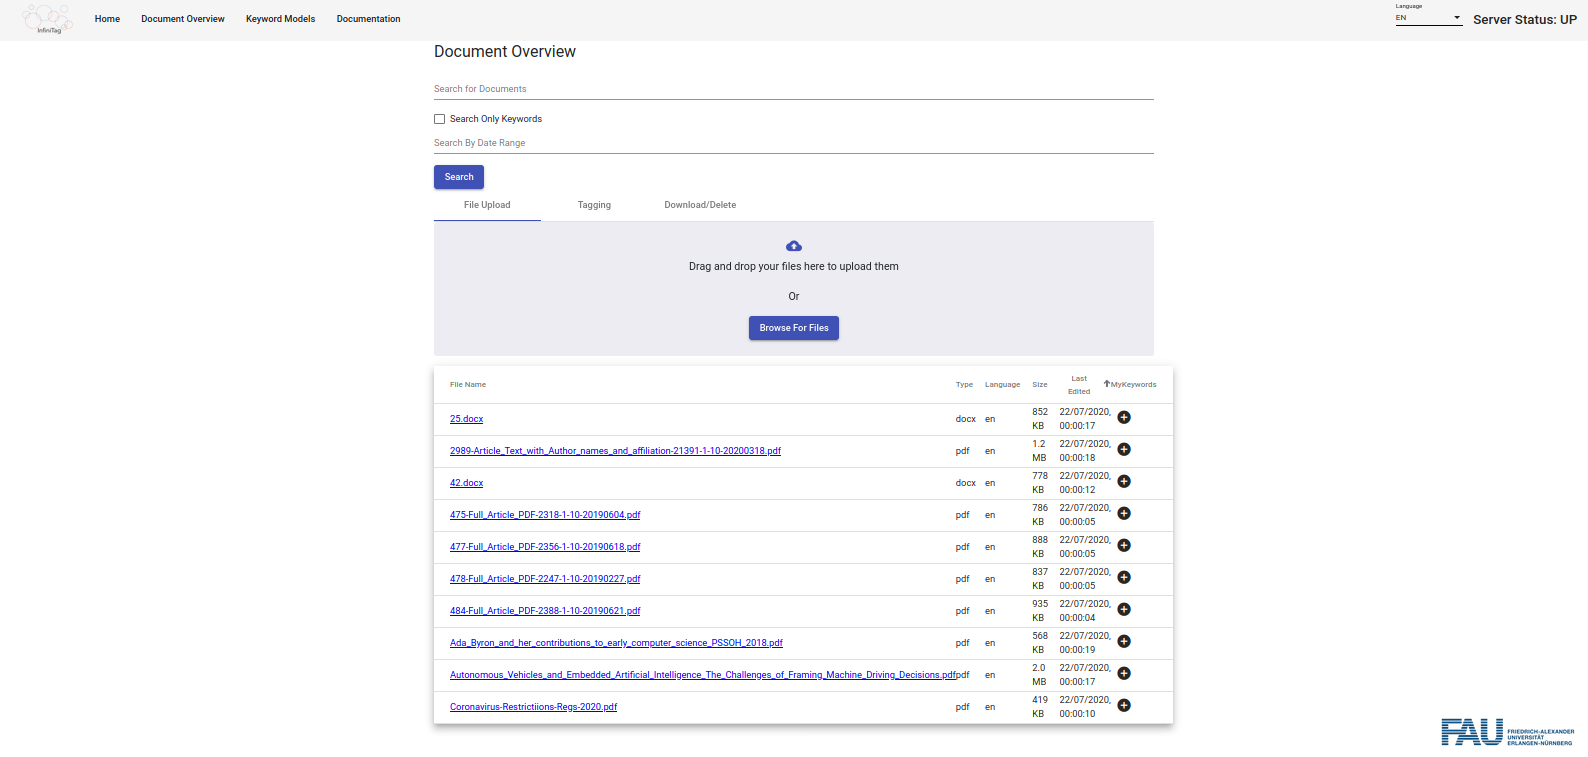
\includegraphics[scale=0.25]{img/doc1.png}
    \caption{The Start page}
    \label{fig:start_page}
\end{figure}

\section{Adding Documents}
Navigating to \verb|\documents| in the browser or clicking on the \verb|Add Documents| link in the menu will take the user to a form where they can select one or more documents to be uploaded. This can be seen in Figure \ref{fig:doc_upload}.

Upon selecting one or more documents all of the documents will be sent to the server for further processing. At the moment the documents will be stored in the database and the meta-information such as name, language, type, etc. will be extracted and stored along with the document content.

\begin{figure}
    \centering
    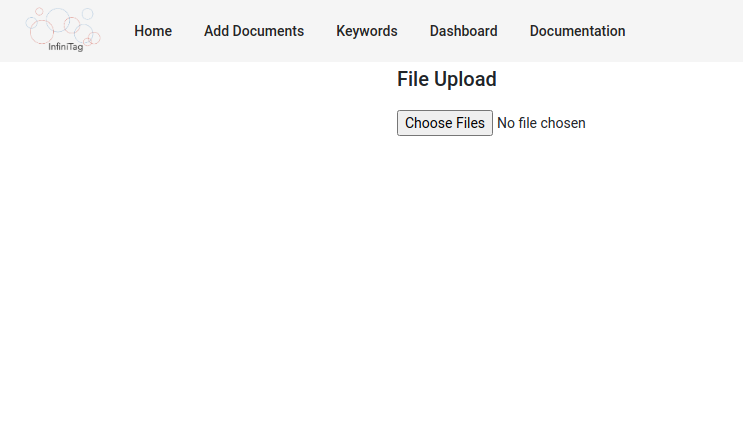
\includegraphics[scale=0.4]{img/doc2.png}
    \caption{Uploading Documents}
    \label{fig:doc_upload}
\end{figure}

\section{Maintaining Keywords}
Navigating to \verb|keywords| or clicking on the \verb|Keywords| link will take the user to a page where they can add dimensions and keywords to a keyword model as seen in Figure \ref{fig:key1}. These keywords are then available to be assigned to the documents on the start / document overview page.

Here one can add dimensions as well as keywords, which will enable the construction of hierarchical keyword models.

\begin{figure}
    \centering
    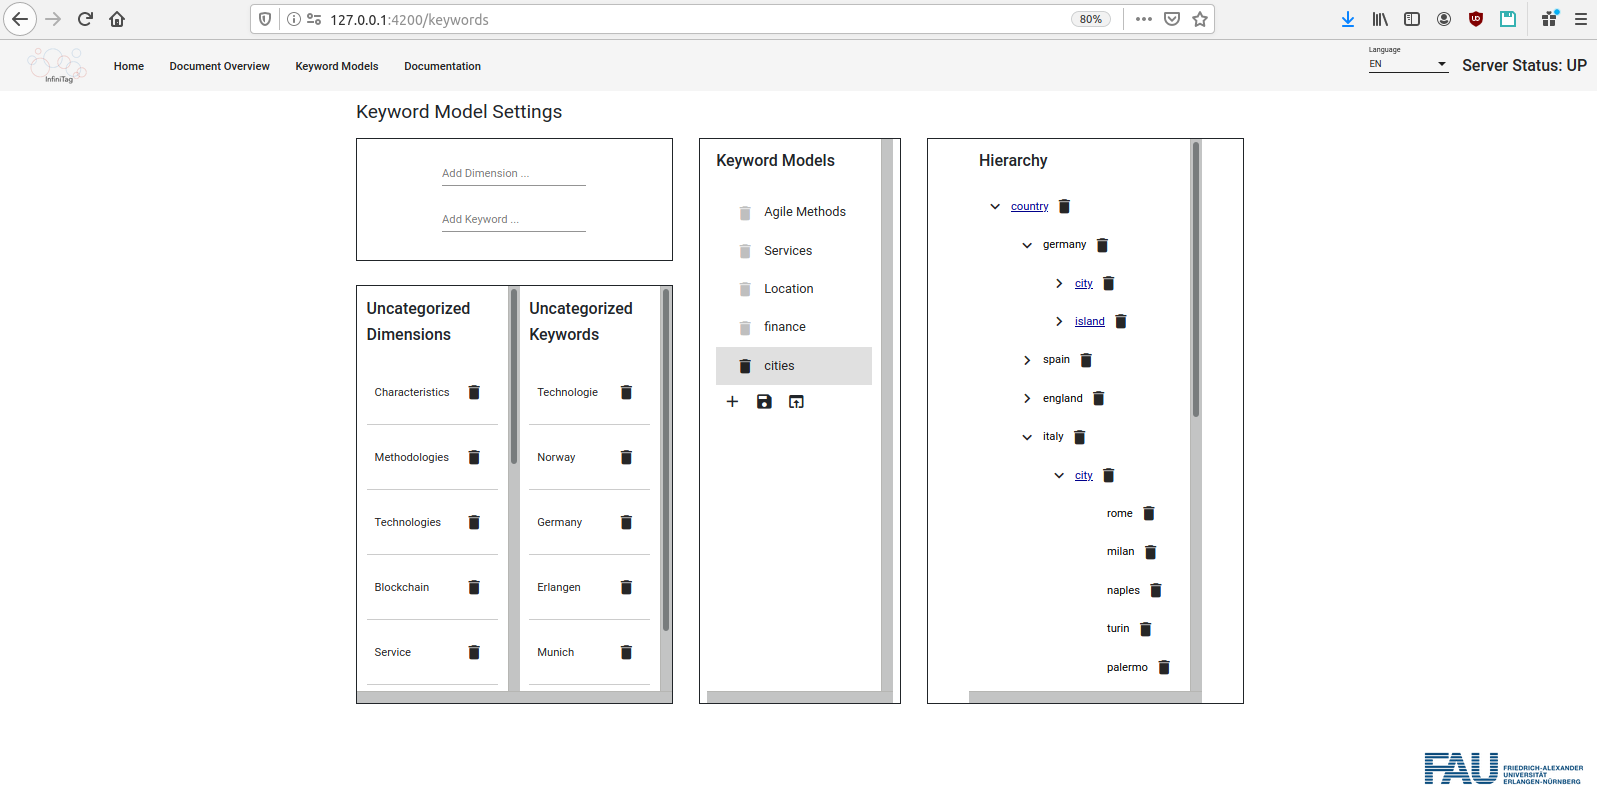
\includegraphics[scale=0.4]{img/key1.png}
    \caption{Maintaining Keywords}
    \label{fig:key1}
\end{figure}

\section{Further Documentation}
Clicking on the \verb|Documentation| link will provide the user with three options as seen in Figure \ref{fig:doc_drop}:

\begin{enumerate}
    \item API Documentation. This provides the user with an overview of all API endpoints for the back end, along with the required parameters and expected return results. A partial example can be seen in Figure \ref{fig:apidoc}
    \item Front End Documentation. This is an external link which will show the user the actual code documentation for the front end.
    \item Back End Documentation. This is another external link which will show the code documentation for the server.
\end{enumerate}

\begin{figure}
    \centering
    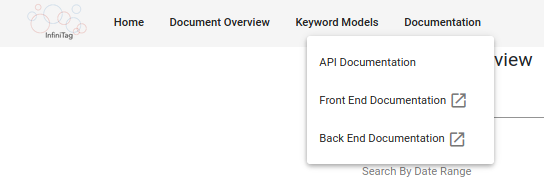
\includegraphics[scale=0.4]{img/doc3.png}
    \caption{Documentation Drop Down}
    \label{fig:doc_drop}
\end{figure}

\begin{figure}
    \centering
    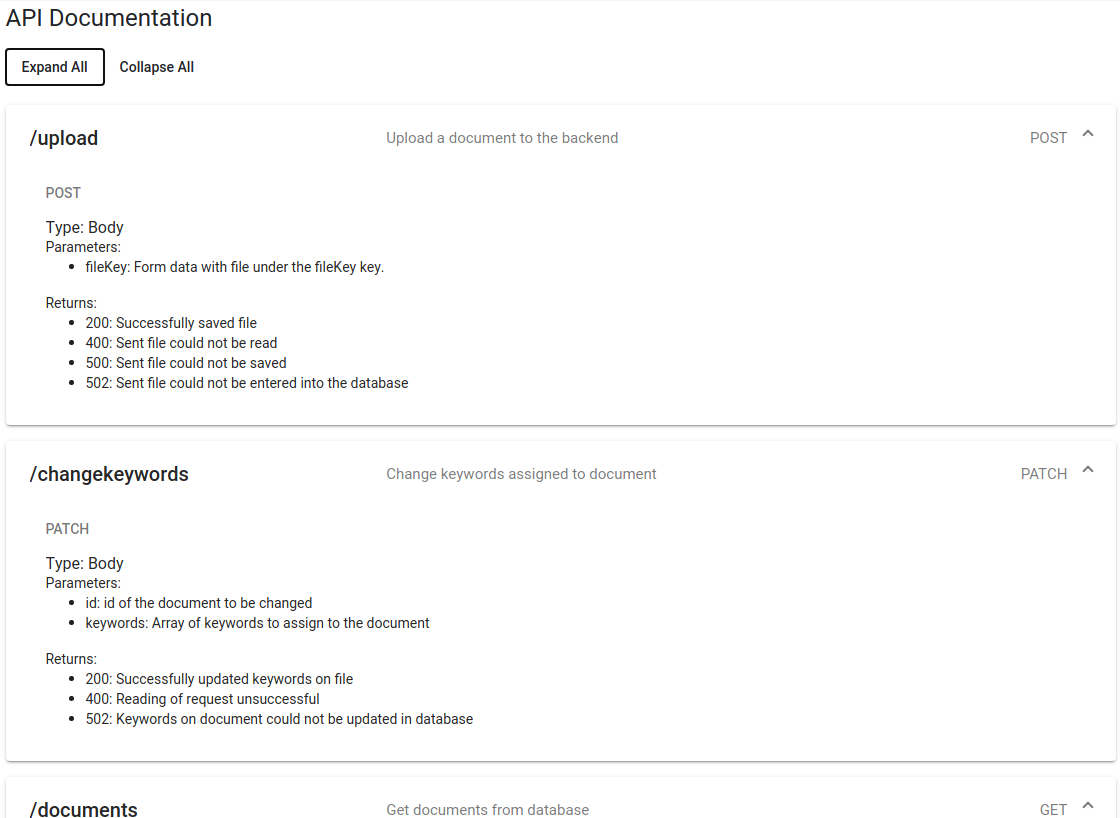
\includegraphics[scale=0.4]{img/api1.png}
    \caption{API Documentation}
    \label{fig:apidoc}
\end{figure}


\section{Utilities}
Important to notice is that the InfiniTag software comes with a utils folder. These are, in part, helper functions for the developers. However much more importantly are the scripts for categorizing and clustering documents. These scripts provide functionality for k-means clustering, hierarchical clustering, LDA, and TF-IDF. These are experimental features which will be integrated into the core solution as soon as possible.

\section{License}
InfiniTag Copyright © 2020 AMOS-5
Permission is hereby granted,
free of charge, to any person obtaining a copy of this software and
associated documentation files (the "Software"), to deal in the Software
without restriction, including without limitation the rights to use, copy,
modify, merge, publish, distribute, sublicense, and/or sell copies of the
Software, and to permit persons to whom the Software is furnished to do so,
subject to the following conditions: The above copyright notice and this
permission notice shall be included in all copies or substantial portions
of the Software. THE SOFTWARE IS PROVIDED "AS IS", WITHOUT WARRANTY OF ANY
KIND, EXPRESS OR IMPLIED, INCLUDING BUT NOT LIMITED TO THE WARRANTIES OF
MERCHANTABILITY, FITNESS FOR A PARTICULAR PURPOSE AND NONINFRINGEMENT. IN
NO EVENT SHALL THE AUTHORS OR COPYRIGHT HOLDERS BE LIABLE FOR ANY CLAIM,
DAMAGES OR OTHER LIABILITY, WHETHER IN AN ACTION OF CONTRACT, TORT OR
OTHERWISE, ARISING FROM, OUT OF OR IN CONNECTION WITH THE SOFTWARE OR THE
USE OR OTHER DEALINGS IN THE SOFTWARE.
\end{document}

